\documentclass[11pt]{article}

% ---- Packages ----
\usepackage[utf8]{inputenc}
\usepackage[T1]{fontenc}
\usepackage{lmodern}
\usepackage[margin=1in]{geometry}
\usepackage{amsmath,amssymb}
\usepackage{graphicx}
\usepackage{booktabs}
\usepackage{hyperref}
\usepackage{xcolor}
\usepackage{listings}
\usepackage{tikz}
\usepackage{pgfplots}
\usepackage{caption}
\usepackage{subcaption}
\usepackage{enumitem}
\usepackage{fancyhdr}
\usepackage{url}
\usepackage{multirow}
\usepackage{needspace}
\usepackage{placeins}

\pgfplotsset{compat=1.18}
\tolerance=1000
\emergencystretch=1em
\usetikzlibrary{positioning, arrows.meta, shapes.geometric, fit, calc}

\hypersetup{
  colorlinks=true,
  linkcolor=blue!70!black,
  citecolor=green!50!black,
  urlcolor=blue!70!black,
}

\lstset{
  basicstyle=\ttfamily\small,
  keywordstyle=\color{blue!70!black}\bfseries,
  commentstyle=\color{green!50!black}\itshape,
  stringstyle=\color{red!60!black},
  breaklines=true,
  frame=single,
  numbers=left,
  numberstyle=\tiny\color{gray},
  xleftmargin=2em,
  framexleftmargin=1.5em,
  tabsize=2,
  showstringspaces=false,
}

% ---- Title ----
\title{\textbf{Exploring Zero-Copy mmap Loading and KV Cache \\ Pre-Allocation for MLX on Apple Silicon}}
\author{
  AtomGradient
}
\date{\today}

\begin{document}

\maketitle

% ============================================================
% Abstract
% ============================================================
\begin{abstract}
llama.cpp achieves remarkably flat memory behavior on Apple Silicon through memory-mapped (mmap) weight loading and pre-allocated KV caches.
We investigate whether these same techniques can benefit the MLX framework, which instead uses \texttt{pread}-based loading and dynamically grown KV caches.
We implement a zero-copy mmap loading path in MLX's C++ core and a KV cache pre-allocation option in mlx-lm, and evaluate both across eight Qwen3 quantized model variants on an M1~Max (32\,GB).
Our results are mixed: mmap loading shows dramatic speedups for certain larger models (up to 20$\times$ for one 8\,GB model) but performs \emph{worse} than standard loading for small models and in some large-model configurations.
KV pre-allocation successfully flattens memory growth but adds 0.5--0.6\,GB of upfront cost and slightly increases first-token latency, offering no throughput benefit over MLX's dynamic approach.
During implementation, we also discovered and fixed a quantized model dtype inference bug.
Overall, our findings suggest that \textbf{MLX's existing memory management is already well-suited to its design goals}, and that naively transplanting llama.cpp's strategies does not yield consistent improvements.
We present our implementation details, benchmark data, and analysis of why these techniques interact differently with MLX's lazy evaluation model.
\end{abstract}

% ============================================================
% 1. Introduction
% ============================================================
\section{Introduction}
\label{sec:intro}

The MLX framework~\cite{mlx2023} by Apple provides a NumPy-like API with lazy evaluation and automatic differentiation, designed for Apple Silicon's Metal GPU backend.
Combined with the mlx-lm inference engine, it has become a popular choice for running large language models (LLMs) locally on Mac hardware.

A separate ecosystem, llama.cpp~\cite{llamacpp}, takes a very different approach to memory management.
It uses memory-mapped file I/O (\texttt{mmap}) for model loading, achieving zero-copy weight access, and pre-allocates the entire KV cache at startup, resulting in flat, predictable memory consumption~\cite{ggml2023}.
In contrast, MLX's default path uses \texttt{pread()} to load safetensors weights into allocated buffers, and its KV cache grows dynamically in 256-token increments.

A natural question arises: \emph{would MLX benefit from adopting llama.cpp's memory strategies?}
In this paper, we explore this question by implementing both techniques within the MLX ecosystem and conducting systematic benchmarks.
Our findings are nuanced:
\begin{itemize}[leftmargin=*]
  \item Mmap loading helps significantly in some configurations but hurts in others, revealing that MLX's \texttt{pread}-based loader is already highly efficient for typical model sizes.
  \item KV pre-allocation achieves its goal of flat memory usage but at the cost of increased startup latency and memory overhead, with no throughput improvement over the dynamic approach.
  \item MLX's lazy evaluation model and the safetensors format introduce constraints (e.g., offset alignment, tensor materialization) that make zero-copy loading less straightforward than in llama.cpp's GGUF-based pipeline.
\end{itemize}

Our specific contributions are:
\begin{enumerate}[leftmargin=*]
  \item \textbf{Mmap loading implementation:} A \texttt{MmapReader} class in MLX's C++ core that memory-maps safetensors files and exposes offset views via Metal buffers, with alignment checks and fallback paths.
  \item \textbf{KV cache pre-allocation:} An optional \texttt{max\_context\_length} parameter for mlx-lm's \texttt{KVCache} that reserves the full context window upfront.
  \item \textbf{Quantized dtype bug fix:} Discovery of a bug where \texttt{Quantized\-Linear.weight.dtype} returns \texttt{uint32} instead of the working precision.
  \item \textbf{Systematic benchmarks and analysis:} Three benchmark suites across eight models, with discussion of \emph{why} these techniques do not consistently outperform MLX's defaults.
\end{enumerate}

% ============================================================
% 2. Background
% ============================================================
\section{Background}
\label{sec:background}

\subsection{Apple Silicon Unified Memory Architecture}
\label{sec:uma}

Apple Silicon processors (M1--M4 series) feature a Unified Memory Architecture (UMA) where CPU, GPU, and Neural Engine share the same physical memory pool with up to 800\,GB/s bandwidth.
This eliminates the traditional PCIe bottleneck, enabling zero-copy data sharing: a buffer allocated once can be accessed by both CPU and GPU without any transfer.

\subsection{The Safetensors Format}
\label{sec:safetensors}

Safetensors~\cite{safetensors} is a simple, safe tensor serialization format by Hugging Face.
A safetensors file contains an 8-byte header length, a JSON header mapping tensor names to their data types, shapes, and byte offsets, followed by the raw tensor data.
The format supports direct byte-offset access, making it amenable to memory-mapped loading.
However, the specification does not guarantee that tensor offsets are aligned to element boundaries (e.g., 2-byte alignment for float16), which complicates zero-copy access.

\subsection{MLX Framework}
\label{sec:mlx}

MLX~\cite{mlx2023} is a machine learning framework for Apple Silicon.
Key design principles include lazy evaluation (operations are recorded into a computation graph and executed only when results are needed), a NumPy-like Python API, and composable function transformations.
The Metal backend compiles operations into GPU compute shaders.
MLX loads model weights via a \texttt{Load} primitive that, by default, uses \texttt{pread()} to read data from disk into a newly allocated buffer.
Notably, this design gives MLX full control over buffer lifecycle and enables optimizations within its lazy evaluation graph that may not be possible with externally managed mmap buffers.

\subsection{KV Cache in LLM Inference}
\label{sec:kv}

Autoregressive LLM inference caches key and value projections to avoid redundant computation.
The cache size grows linearly with sequence length: for a model with $L$ layers, $H$ KV heads, and head dimension $d$, storing $T$ tokens requires $2 \times L \times H \times T \times d$ elements.
In mlx-lm's default implementation, the cache starts empty and grows in 256-token chunks.
While this ``staircase'' growth pattern uses more memory management operations, it has the advantage of allocating only the memory actually needed.

\subsection{How llama.cpp Differs}
\label{sec:llamacpp}

llama.cpp~\cite{llamacpp} takes a fundamentally different approach.
It uses \texttt{mmap} to map GGUF model files directly into the process address space, relying on the OS page cache for demand paging.
Its static computation graph (\texttt{ggml}) pre-analyzes all tensor dependencies and uses a graph-coloring memory allocator to maximize buffer reuse~\cite{ggml2023}.
The KV cache is allocated at full context length at startup.
These design choices yield nearly constant memory consumption during inference---but they are tightly coupled to GGUF's guaranteed-aligned format and ggml's ahead-of-time memory planning, neither of which directly applies to MLX's safetensors-based, lazy-evaluation pipeline.

% ============================================================
% 3. Design & Implementation
% ============================================================
\section{Implementation}
\label{sec:design}

\subsection{Zero-Copy mmap Loading}
\label{sec:mmap}

\subsubsection{Architecture}

Figure~\ref{fig:mmap_arch} illustrates the mmap loading path.
When \texttt{mx.load(path,\allowbreak{} use\_mmap=True)} is called, the Python binding constructs an \texttt{Mmap\-Reader} instead of the default \texttt{Parallel\-File\-Reader}.

\begin{figure}[t]
\centering
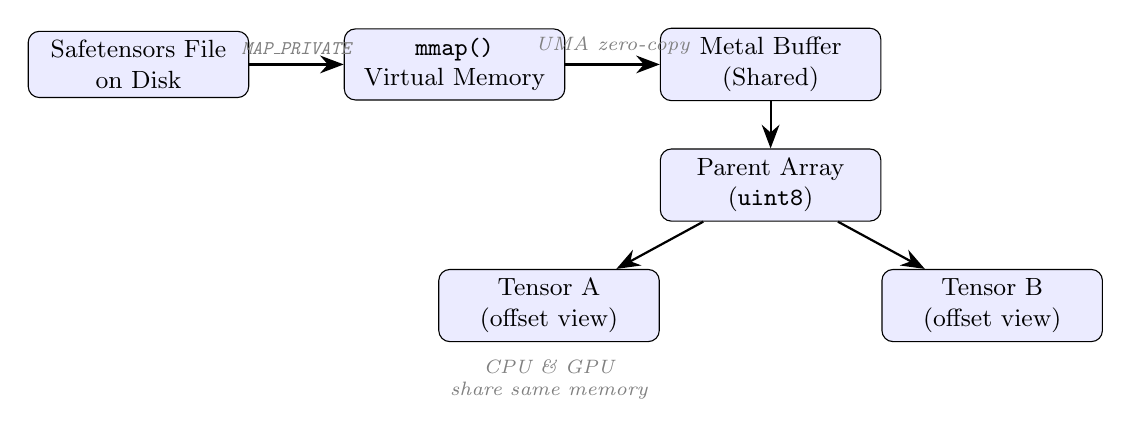
\begin{tikzpicture}[
  node distance=0.6cm and 1.2cm,
  block/.style={rectangle, draw, rounded corners, fill=blue!8,
    minimum width=2.8cm, minimum height=0.8cm, align=center, font=\small},
  arrow/.style={-{Stealth[length=3mm]}, thick},
  label/.style={font=\scriptsize\itshape, text=gray}
]
  \node[block] (file) {Safetensors File\\on Disk};
  \node[block, right=of file] (mmap) {\texttt{mmap()}\\Virtual Memory};
  \node[block, right=of mmap] (metal) {Metal Buffer\\(Shared)};
  \node[block, below=of metal] (parent) {Parent Array\\(\texttt{uint8})};
  \node[block, below left=0.6cm and 0cm of parent] (view1) {Tensor A\\(offset view)};
  \node[block, below right=0.6cm and 0cm of parent] (view2) {Tensor B\\(offset view)};
  \draw[arrow] (file) -- (mmap) node[midway, above, label] {\texttt{MAP\_PRIVATE}};
  \draw[arrow] (mmap) -- (metal) node[midway, above, label] {UMA zero-copy};
  \draw[arrow] (metal) -- (parent);
  \draw[arrow] (parent) -- (view1);
  \draw[arrow] (parent) -- (view2);
  \node[label, below=0.1cm of view1, text width=3cm, align=center] {CPU \& GPU\\share same memory};
\end{tikzpicture}
\caption{Mmap loading data flow. The safetensors file is memory-mapped once; a Metal buffer is created over the mapped region. Individual tensors are exposed as offset views into a parent array.}
\label{fig:mmap_arch}
\end{figure}

\subsubsection{MmapReader}

The \texttt{MmapReader} class (Listing~1) encapsulates the POSIX mmap lifecycle.
The file descriptor is opened, the file is mapped into virtual memory with \texttt{MAP\_PRIVATE} (copy-on-write semantics), and the descriptor is immediately closed---the mapping persists independently.
The \texttt{MADV\_SEQUENTIAL} hint enables kernel readahead for sequential tensor access.
A Metal buffer is then lazily created over the mmap region via \texttt{allocator::make\_buffer()}, exploiting UMA for zero-copy GPU access.

\begin{lstlisting}[language=C++, caption={MmapReader constructor (simplified).}, float=tp]
MmapReader::MmapReader(std::string file_path) {
  int fd = open(file_path.c_str(), O_RDONLY);
  struct stat st;
  fstat(fd, &st);
  file_size_ = st.st_size;
  mmap_ptr_ = mmap(nullptr, file_size_,
    PROT_READ, MAP_PRIVATE, fd, 0);
  close(fd);  // mmap survives fd closure
  madvise(mmap_ptr_, file_size_, MADV_SEQUENTIAL);
}
\end{lstlisting}

\subsubsection{Alignment Check and Fallback}

The critical zero-copy path in \texttt{Load::eval\_cpu()} (Listing~2) creates offset views into the mmap buffer, but requires a careful alignment check.

\begin{lstlisting}[language=C++, caption={Zero-copy path with alignment guard (simplified).}, float=tp]
if (reader_->is_mmap() && !swap_endianness_) {
  auto mmap_reader = dynamic_pointer_cast<MmapReader>(reader_);
  if (mmap_reader && (offset_ % out.itemsize() == 0)) {
    auto metal_buf = mmap_reader->get_metal_buffer();
    auto parent = array(metal_buf, {1}, uint8,
      [reader_ref](Buffer) { /* prevent dealloc */ });
    out.copy_shared_buffer(parent, strides, flags,
      out.size(), offset_ / out.itemsize());
    return;  // Zero-copy success
  }
}
// Fallback: allocate + memcpy for unaligned offsets
\end{lstlisting}

The check \texttt{offset\_ \% out.itemsize() == 0} is essential because safetensors does not guarantee element-aligned offsets.
Without it, integer division would silently truncate the byte offset, corrupting tensor data.
The lifecycle of the \texttt{MmapReader} is managed by capturing a \texttt{shared\_ptr<Reader>} in the parent array's deleter lambda, ensuring the mapping persists as long as any tensor references it.

\subsection{KV Cache Pre-Allocation}
\label{sec:prealloc}

In MLX's default implementation, the KV cache starts as \texttt{None} and grows in 256-token steps.
Each expansion allocates a new buffer and copies existing data, producing the staircase pattern shown in Figure~\ref{fig:kv_comparison}.
Our pre-allocation approach reserves the full context window at startup, yielding a flat memory profile at the cost of higher initial usage.

\begin{figure}[t]
\centering
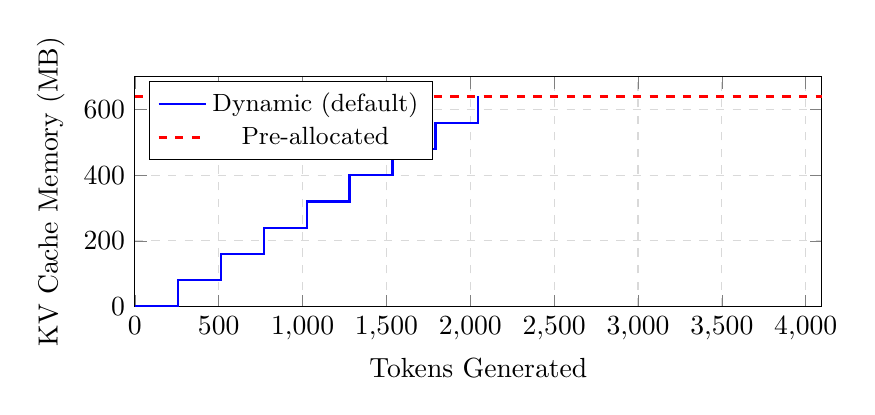
\begin{tikzpicture}
\begin{axis}[
  width=0.85\columnwidth,
  height=4.5cm,
  xlabel={Tokens Generated},
  ylabel={KV Cache Memory (MB)},
  xmin=0, xmax=4096,
  ymin=0, ymax=700,
  legend style={at={(0.02,0.98)}, anchor=north west, font=\small},
  grid=major,
  grid style={dashed, gray!30},
]
  \addplot[blue, thick, const plot] coordinates {
    (0,0) (256,80) (512,160) (768,240) (1024,320)
    (1280,400) (1536,480) (1792,560) (2048,640)
  };
  \addlegendentry{Dynamic (default)}

  \addplot[red, thick, dashed] coordinates {
    (0,640) (4096,640)
  };
  \addlegendentry{Pre-allocated}
\end{axis}
\end{tikzpicture}
\caption{KV cache memory over time: dynamic growth vs.\ pre-allocation. Pre-allocation provides flat memory at the cost of higher initial usage.}
\label{fig:kv_comparison}
\end{figure}

\FloatBarrier

\subsubsection{Implementation}

Pre-allocation is controlled by three parameters added to the \texttt{KVCache} constructor: \texttt{n\_kv\_heads}, \texttt{head\_dim}, and \texttt{max\_context\_length}.
All default to zero, ensuring full backward compatibility---existing code without these parameters continues to use dynamic growth.
When all three are positive, the constructor allocates keys and values tensors for the full context length, aligned to the 256-token step boundary.
The \texttt{mx.eval()} call forces immediate physical allocation, bypassing MLX's lazy evaluation.
If the sequence later exceeds the pre-allocated length, the cache gracefully falls back to dynamic expansion via concatenation.
Listing~3 shows the simplified implementation.

\begin{lstlisting}[language=Python, caption={KVCache pre-allocation (simplified).}, float=tp]
class KVCache(_BaseCache):
    step = 256
    def __init__(self, n_kv_heads=0, head_dim=0,
                 max_context_length=0, dtype=mx.float16):
        self.offset = 0
        if max_context_length > 0 and n_kv_heads > 0:
            L = ((max_context_length + 255) // 256) * 256
            self.keys = mx.zeros(
                (1, n_kv_heads, L, head_dim), dtype=dtype)
            self.values = mx.zeros(
                (1, n_kv_heads, L, head_dim), dtype=dtype)
            mx.eval(self.keys, self.values)  # Force alloc
\end{lstlisting}

\subsection{Quantized Model dtype Bug}
\label{sec:dtype_fix}

During implementation, we discovered that \texttt{QuantizedLinear.weight.dtype} returns \texttt{uint32} (the packed storage type) rather than the model's working precision.
This caused the KV cache to be allocated in \texttt{uint32} instead of \texttt{float16}.
The fix inspects the \texttt{scales} tensor for quantized layers, which stores dequantization factors in the correct working dtype.

% ============================================================
% 4. Evaluation
% ============================================================
\section{Evaluation}
\label{sec:eval}

\subsection{Setup}
\label{sec:setup}

\begin{itemize}[leftmargin=*]
  \item \textbf{Hardware:} Apple M1~Max, 32\,GB unified memory
  \item \textbf{Software:} macOS, MLX 0.30.7, Python 3.11
  \item \textbf{Models:} Eight Qwen3~\cite{qwen3} quantized variants (Table~\ref{tab:models})
  \item \textbf{Prompt:} 34-token fixed physics question; 200 output tokens per run
\end{itemize}

\begin{table}[t]
\centering
\caption{Model variants used in benchmarks.}
\label{tab:models}
\small
\begin{tabular}{lrr}
\toprule
\textbf{Model} & \textbf{Parameters} & \textbf{Size (GB)} \\
\midrule
Qwen3-4B-4bit  & 4B  & 2.11 \\
Qwen3-4B-8bit  & 4B  & 3.98 \\
Qwen3-8B-3bit  & 8B  & 3.34 \\
Qwen3-8B-4bit  & 8B  & 4.29 \\
Qwen3-8B-6bit  & 8B  & 6.20 \\
Qwen3-8B-8bit  & 8B  & 8.11 \\
Qwen3-14B-4bit & 14B & 7.74 \\
Qwen3-14B-6bit & 14B & 11.18 \\
\bottomrule
\end{tabular}
\end{table}

\subsection{Loading Speed}
\label{sec:loading}

Table~\ref{tab:loading} and Figure~\ref{fig:loading_bar} compare loading times (3 runs each, page cache warmed).

\begin{table}[t]
\centering
\caption{Model loading time: standard vs.\ mmap (seconds). Speedup $>1$ means mmap is faster; $<1$ means mmap is \emph{slower}.}
\label{tab:loading}
\small
\begin{tabular}{lrrr}
\toprule
\textbf{Model} & \textbf{Standard (s)} & \textbf{Mmap (s)} & \textbf{Speedup} \\
\midrule
Qwen3-4B-4bit  & 0.101 & 0.131 & 0.77$\times$ \\
Qwen3-4B-8bit  & 0.184 & 0.246 & 0.75$\times$ \\
Qwen3-8B-3bit  & 0.146 & 0.075 & 1.95$\times$ \\
Qwen3-8B-4bit  & 0.352 & 0.328 & 1.07$\times$ \\
Qwen3-8B-6bit  & 0.637 & 0.435 & 1.46$\times$ \\
Qwen3-8B-8bit  & 2.572 & 0.125 & 20.65$\times$ \\
Qwen3-14B-4bit & 2.323 & 0.535 & 4.34$\times$ \\
Qwen3-14B-6bit & 3.701 & 5.388 & 0.69$\times$ \\
\bottomrule
\end{tabular}
\end{table}

\begin{figure}[t]
\centering
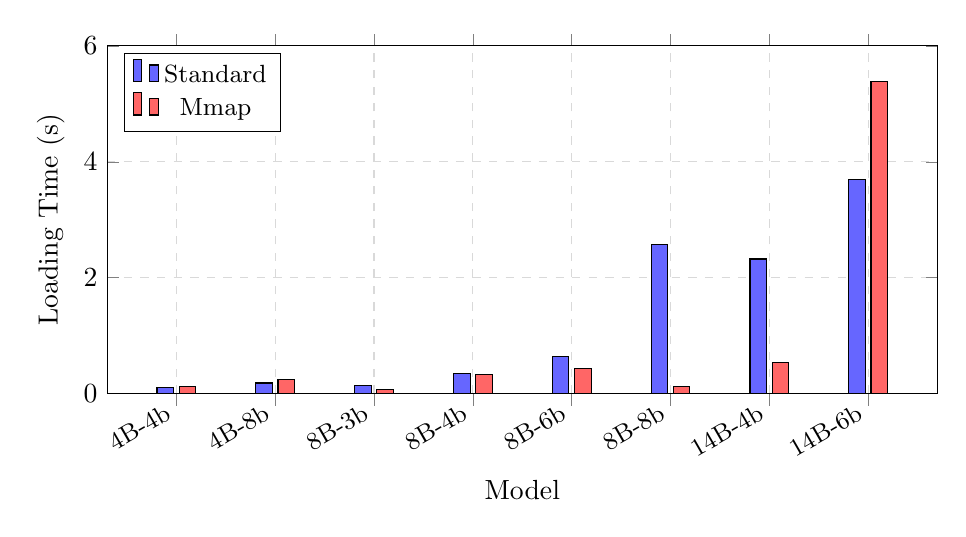
\begin{tikzpicture}
\begin{axis}[
  ybar,
  width=\columnwidth,
  height=6cm,
  bar width=6pt,
  xlabel={Model},
  ylabel={Loading Time (s)},
  symbolic x coords={4B-4b, 4B-8b, 8B-3b, 8B-4b, 8B-6b, 8B-8b, 14B-4b, 14B-6b},
  xtick=data,
  x tick label style={rotate=30, anchor=east, font=\small},
  ymin=0, ymax=6,
  legend style={at={(0.02,0.98)}, anchor=north west, font=\small},
  grid=major,
  grid style={dashed, gray!30},
]
  \addplot[fill=blue!60] coordinates {
    (4B-4b, 0.101) (4B-8b, 0.184) (8B-3b, 0.146) (8B-4b, 0.352)
    (8B-6b, 0.637) (8B-8b, 2.572) (14B-4b, 2.323) (14B-6b, 3.701)
  };
  \addlegendentry{Standard}

  \addplot[fill=red!60] coordinates {
    (4B-4b, 0.131) (4B-8b, 0.246) (8B-3b, 0.075) (8B-4b, 0.328)
    (8B-6b, 0.435) (8B-8b, 0.125) (14B-4b, 0.535) (14B-6b, 5.388)
  };
  \addlegendentry{Mmap}
\end{axis}
\end{tikzpicture}
\caption{Loading time comparison. Results are highly variable: mmap helps for some models (8B-8bit) but is slower for others (4B-4bit, 4B-8bit, 14B-6bit).}
\label{fig:loading_bar}
\end{figure}

The results are \textbf{inconsistent across models}.
Three out of eight models (4B-4bit, 4B-8bit, 14B-6bit) load \emph{slower} with mmap.
The 20.65$\times$ speedup on Qwen3-8B-8bit is an outlier---possibly due to the standard loader hitting a pathological \texttt{pread} pattern for this specific file layout.
For the majority of models in the 2--6\,GB range, the difference is small (0.75--1.46$\times$), suggesting that MLX's standard loading is already efficient enough that mmap offers limited benefit.

\subsection{Inference Impact}
\label{sec:inference}

Table~\ref{tab:inference} examines whether the loading method affects runtime inference.

\begin{table}[t]
\centering
\caption{Inference performance with standard vs.\ mmap loading. Generation throughput (Gen t/s) is the metric most relevant to user experience.}
\label{tab:inference}
\small
\setlength{\tabcolsep}{3pt}
\begin{tabular}{l rr rr rr rr}
\toprule
& \multicolumn{2}{c}{\textbf{Load (s)}} & \multicolumn{2}{c}{\textbf{Prompt (t/s)}} & \multicolumn{2}{c}{\textbf{Gen (t/s)}} & \multicolumn{2}{c}{\textbf{Mem (GB)}} \\
\cmidrule(lr){2-3} \cmidrule(lr){4-5} \cmidrule(lr){6-7} \cmidrule(lr){8-9}
\textbf{Model} & Std & Mmap & Std & Mmap & Std & Mmap & Std & Mmap \\
\midrule
4B-4bit  & 0.89 & 0.85 & 189.1 & 188.6 & 56.9 & 58.5 & 2.38 & 2.38 \\
4B-8bit  & 1.31 & 0.98 & 165.8 & 159.7 & 41.0 & 42.0 & 4.37 & 4.37 \\
8B-3bit  & 1.22 & 0.69 & 100.8 & 92.3  & 29.9 & 29.4 & 4.37 & 4.37 \\
8B-4bit  & 1.34 & 1.03 & 89.8  & 100.7 & 30.1 & 30.1 & 4.72 & 8.82$^\dagger$ \\
8B-6bit  & 2.00 & 1.29 & 86.7  & 75.7  & 20.7 & 20.7 & 8.82 & 8.82 \\
8B-8bit  & 3.04 & 0.77 & 64.4  & 80.6  & 21.6 & 21.3 & 8.82 & 8.84 \\
14B-4bit & 1.95 & 1.01 & 43.4  & 43.2  & 16.2 & 16.5 & 8.84 & 11.09$^\dagger$ \\
14B-6bit & 3.41 & 3.07 & 39.7  & 37.0  & 12.1 & 12.0 & 12.08 & 12.16 \\
\bottomrule
\end{tabular}
\vspace{2pt}
\small{$^\dagger$ Memory nearly doubled---mmap region likely coexists with materialized copies.}
\end{table}

Two findings stand out:
\begin{itemize}[leftmargin=*]
  \item \textbf{Generation throughput is unchanged.} Across all eight models, the generation speed difference is within noise ($<$3\%), confirming that loading method does not affect runtime performance.
  This is expected: once weights are in memory, the computation is identical.
  \item \textbf{Mmap can \emph{increase} peak memory.} For 8B-4bit and 14B-4bit ($\dagger$), peak memory nearly doubled with mmap.
  This suggests that when MLX materializes quantized tensors during lazy evaluation, it allocates new buffers while the mmap-backed originals remain pinned---\emph{the opposite of the memory saving we hoped for}.
\end{itemize}

\subsection{KV Cache Pre-Allocation}
\label{sec:prealloc_eval}

Table~\ref{tab:prealloc} shows results for three models across dynamic, 2048-token, and 4096-token pre-allocation.

\begin{table}[t]
\centering
\caption{KV cache pre-allocation impact. FTLT = first token latency (ms).}
\label{tab:prealloc}
\small
\setlength{\tabcolsep}{3.5pt}
\begin{tabular}{ll rrrr r}
\toprule
\textbf{Model} & \textbf{Mode} & \textbf{FTLT} & \textbf{Prompt} & \textbf{Gen} & \textbf{Peak} & $\Delta$\textbf{Mem} \\
& & (ms) & (t/s) & (t/s) & (GB) & (GB) \\
\midrule
\multirow{3}{*}{4B-4bit}
  & Dynamic      & 260.4 & 200.4 & 62.0 & 2.221 & --- \\
  & Pre-alloc 2k & 276.2 & 183.5 & 63.0 & 2.471 & +0.250 \\
  & Pre-alloc 4k & 285.2 & 171.9 & 62.3 & 2.736 & +0.515 \\
\midrule
\multirow{3}{*}{8B-4bit}
  & Dynamic      & 419.2 & 100.5 & 31.3 & 4.395 & --- \\
  & Pre-alloc 2k & 428.0 & 99.1  & 30.3 & 4.633 & +0.238 \\
  & Pre-alloc 4k & 436.1 & 98.0  & 29.7 & 4.908 & +0.513 \\
\midrule
\multirow{3}{*}{14B-4bit}
  & Dynamic      & 859.6 & 44.1  & 16.7 & 7.827 & --- \\
  & Pre-alloc 2k & 917.4 & 41.1  & 16.0 & 8.101 & +0.274 \\
  & Pre-alloc 4k & 901.5 & 41.7  & 16.1 & 8.414 & +0.587 \\
\bottomrule
\end{tabular}
\end{table}

The results show that pre-allocation \textbf{does not improve throughput}:
\begin{itemize}[leftmargin=*]
  \item \textbf{Generation speed is essentially unchanged} ($<$5\% difference), indicating that MLX's dynamic 256-token growth does not cause meaningful overhead during inference.
  \item \textbf{Prompt processing decreases} by 4--14\%, likely because the larger upfront allocation reduces available memory for MLX's computation buffers.
  \item \textbf{First token latency increases} by 5--7\% due to the forced \texttt{mx.eval()} at startup.
  \item \textbf{Memory overhead is predictable:} 0.25\,GB for 2048 tokens, 0.5\,GB for 4096 tokens.
\end{itemize}

The one benefit---flat memory profile---is real but comes at a cost.
MLX's dynamic approach, while producing staircase-like growth, avoids wasting memory for conversations that never reach the pre-allocated context length.

% ============================================================
% 5. Discussion
% ============================================================
\section{Discussion}
\label{sec:discussion}

\subsection{Why MLX's Existing Design Works Well}

Our results paint a clear picture: \textbf{MLX's \texttt{pread}-based loading and dynamic KV cache are more appropriate for its design than we initially expected.}
Several factors explain this:

\paragraph{pread is fast enough.}
For models under 4\,GB (the majority of quantized models people run locally), standard loading completes in under 200\,ms.
At this scale, mmap's overhead---VMA creation, page table setup, TLB pressure---outweighs any benefit from avoiding copies.
MLX's parallel file reader already uses efficient buffered I/O\@.

\paragraph{Lazy evaluation conflicts with mmap.}
MLX's lazy evaluation model means that tensor operations are deferred until explicitly evaluated.
When quantized tensors loaded via mmap are later materialized (e.g., dequantization), MLX allocates \emph{new} buffers for the results while the mmap-backed originals remain referenced.
This can lead to memory \emph{doubling} rather than saving---the exact opposite of our goal.
In contrast, llama.cpp's eager, static graph avoids this issue entirely.

\paragraph{Dynamic KV growth is not a bottleneck.}
We hypothesized that the 256-token step growth pattern would cause allocation overhead and fragmentation.
In practice, the impact is negligible: generation throughput is identical whether the cache is pre-allocated or not.
MLX's allocator handles the periodic growth efficiently.

\subsection{When Mmap Does Help}

Despite the mixed overall results, mmap loading showed dramatic improvements in specific cases: 20.65$\times$ for Qwen3-8B-8bit and 4.34$\times$ for Qwen3-14B-4bit.
These outliers share a common pattern: the standard loader's load time was anomalously high (2.3--2.6\,s for files that ``should'' load faster given their size), suggesting the \texttt{pread} path hit edge cases in the OS I/O scheduler.
This indicates that mmap could serve as a useful fallback for specific problematic file layouts, but not as a general replacement.

\subsection{The 14B-6bit Anomaly}

The largest model tested (11.18\,GB) loaded \emph{slower} with mmap (0.69$\times$).
At this size, the mmap approach must fault in an extremely large number of pages.
The OS page fault handler becomes the bottleneck, as each 16\,KB page requires a kernel trap, page table update, and TLB insertion.
The standard loader's buffered reads, which batch these operations, prove more efficient at scale.

\subsection{Recommendations}

Based on our findings:
\begin{itemize}[leftmargin=*]
  \item \textbf{For most users,} MLX's default loading and dynamic KV cache are the best choice.
  They are fast, memory-efficient, and well-integrated with the lazy evaluation model.
  \item \textbf{Mmap loading} may be useful as an opt-in for specific large models where standard loading is slow, but should not be the default.
  \item \textbf{KV pre-allocation} is only worth considering for server deployments where memory predictability is valued over efficiency, or for long-context scenarios ($>$8k tokens) where avoiding repeated reallocation becomes more important.
\end{itemize}

% ============================================================
% 6. Related Work
% ============================================================
\section{Related Work}
\label{sec:related}

\paragraph{llama.cpp and ggml.}
llama.cpp~\cite{llamacpp} pioneered mmap for LLM weight loading, combined with ggml's static graph and memory-reuse allocator~\cite{ggml2023}.
Our work attempts to bring these techniques to MLX and finds that the benefits are architecture-dependent: what works well for ggml's static pipeline does not automatically transfer to MLX's lazy evaluation model.

\paragraph{vLLM.}
vLLM~\cite{kwon2023vllm} introduced PagedAttention for multi-tenant KV cache management.
Our simpler pre-allocation targets single-user inference but arrives at a similar conclusion: careful memory management has tradeoffs that depend heavily on the workload.

\paragraph{TensorRT-LLM.}
NVIDIA's TensorRT-LLM~\cite{tensorrtllm} uses aggressive pre-allocated KV caches for deterministic memory.
Like our findings, this approach trades flexibility for predictability.

\paragraph{FlashAttention.}
FlashAttention~\cite{dao2022flashattention} reduces per-step attention memory.
This is complementary to our work: it optimizes the computation, while we explore the allocation strategy.

% ============================================================
% 7. Conclusion
% ============================================================
\section{Conclusion}
\label{sec:conclusion}

We explored whether llama.cpp's memory management strategies---mmap loading and KV cache pre-allocation---could improve MLX's performance on Apple Silicon.
Our systematic benchmarks across eight models reveal that these techniques yield \textbf{inconsistent results}: mmap loading helps for some larger models but hurts for small models and can increase peak memory due to interactions with MLX's lazy evaluation; KV pre-allocation achieves flat memory usage but offers no throughput benefit and adds startup overhead.

These findings lead us to a perhaps surprising conclusion: \textbf{MLX's existing memory management---\texttt{pread}-based loading with dynamic KV cache growth---is already well-designed for its target use case.}
The design choices that differ from llama.cpp are not oversights but rather appropriate adaptations to MLX's lazy evaluation model and the safetensors ecosystem.

We hope this exploration is useful to others considering similar optimizations, and that our benchmark data and implementation details serve as a reference.
During this work, we also identified and fixed a quantized model dtype inference bug, which we consider the most practically useful contribution of this project.

All code and benchmark data are available at \url{https://github.com/AtomGradient/OptMLX}.

% ============================================================
% References
% ============================================================
\bibliographystyle{plain}
\bibliography{references}

\end{document}
